% start preamble -------------------------------------------------------------
\documentclass{article}
\usepackage{amsmath, amsthm, amssymb, amsfonts}
\usepackage{thmtools}
\usepackage{graphicx}
\usepackage{setspace}
\usepackage{geometry}
\usepackage{float}
\usepackage{hyperref}
\usepackage[utf8]{inputenc}
\usepackage[english]{babel}
\usepackage{framed}
\usepackage[dvipsnames]{xcolor}
\usepackage{tcolorbox}
\usepackage{ dsfont }
\usepackage{ wasysym }
\usepackage[math]{cellspace}

\setlength\cellspacetoplimit{3pt}
\setlength\cellspacebottomlimit{3pt}
\colorlet{LightGray}{White!90!Periwinkle}
\colorlet{LightOrange}{Orange!15}
\colorlet{LightGreen}{Green!15}

\graphicspath{ {./pictures/} }

\newcommand{\HRule}[1]{\rule{\linewidth}{#1}}

% end preamble -------------------------------------------------------------------

\begin{document}

% ------------------------------------------------------------------------------
% Cover Page and ToC
% ------------------------------------------------------------------------------

\title{ \normalsize \textsc{}
		\\ [2.0cm]
		\HRule{1.5pt} \\
		\LARGE \textbf{\uppercase{ Mathe 2 Hausübung Nr. 6 }
        \HRule{2.0pt} \\ [0.6cm] \LARGE{ Sebastian Steitz, Hannes Albert } \vspace*{10\baselineskip}}
		}
\date{date}
\author{\textbf{} \\
		Gruppe: 6 \\
		Tutor:  Zidane Bührmann}

\maketitle
\setlength\leftskip{1cm}

\section{H6.1}
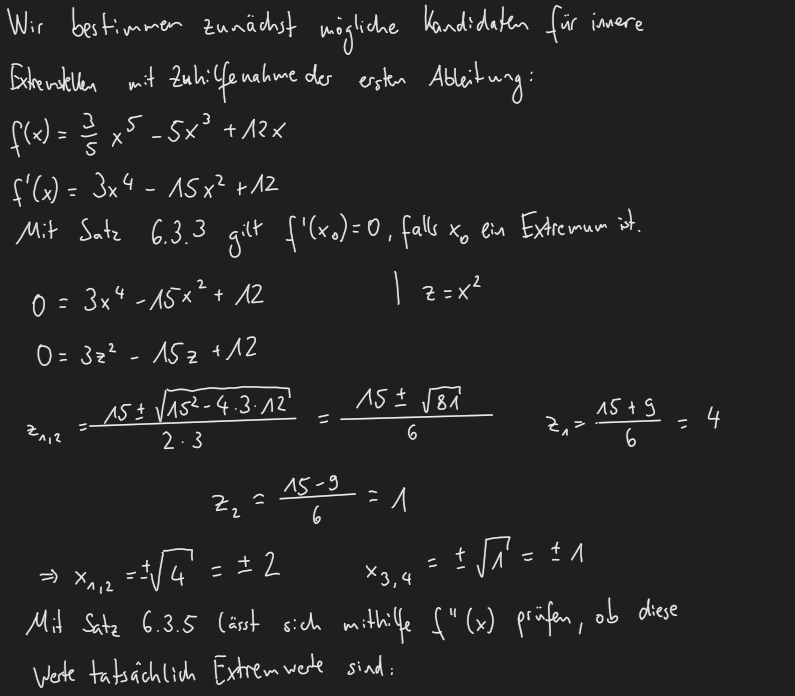
\includegraphics[scale=0.6]{ h1_1 }  

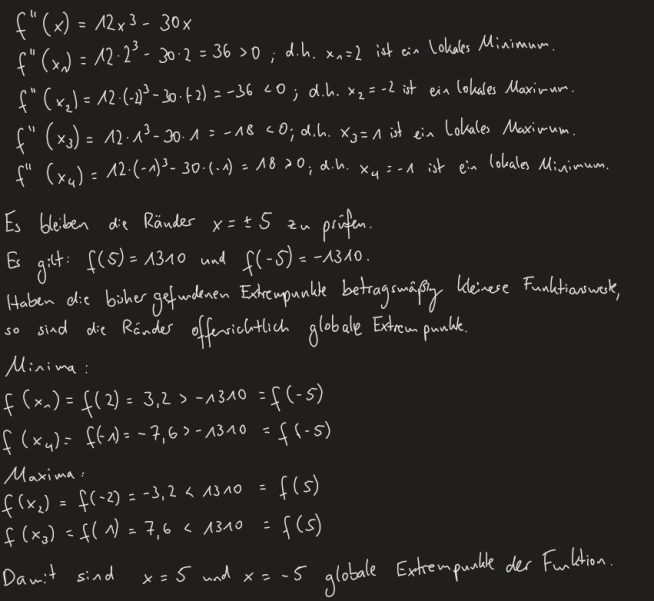
\includegraphics[scale=0.6]{ h1_2 }
\section{H6.2}
\noindent a) \\
Um die Stetigkeit der Funktion zu zeigen, richten wir uns nach Bemerkung 
5.7.13. Es gilt:
\[
    \lim\limits_{x \to (0, 0)} f(x) = 0 = f(0,0) = 0 = f(\lim\limits_{x \to (0, 0)} x)
\]
Somit gilt nach der Bemerkung die Stetigkeit von f in Punkt (0, 0).

\bigskip
\noindent b) \\ 
Wir setzen ein:
\begin{align*}
    \partial_u f(0, 0) &= \lim\limits_{h \to 0} \frac{f(0, 0) + h* u) - f(0, 0)}{h} \\ 
                       &= \lim\limits_{h \to 0} \frac{1}{h} f(h * u) \\ 
                       &= \lim\limits_{h \to 0} \frac{1}{h} f(h * u_1, h * u_2) \\ 
                        &= \lim\limits_{h \to 0} \frac{1}{h} \frac{(h * u_2)^3}{(h * u_1)^2 + (h * u_2)^2} \\ 
                        &= \lim\limits_{h \to 0} \frac{1}{h} \frac{h^3 * u_2^3}{h^2 * u_1^2 + h^2 * u_2^2} \\ 
                        &= \lim\limits_{h \to 0} \frac{h^3 * u_2^3}{h^3 * u_1^2 + h^3 * u_2^2} \\ 
                        &= \lim\limits_{h \to 0} \frac{u_2^3}{h^3 * u_1^2 + h^3 * u_2^2} \\ 
                        &= \lim\limits_{h \to 0} \frac{u_2^3}{u_1^2 + u_2^2} \\ 
                        &= \frac{u_2^3}{u_1^2 + u_2^2} \\ 
                        &= \frac{u_2^3}{\left|| u \right||} \\ 
                        &= \frac{u_2^3}{1} \\ 
                        &= u_2^3
 \end{align*}
 Somit gilt ($\partial_u$f)(0, 0) = $u_2^3$. Insbesondere gibt es keinen Wert, so dass 
 die Richtungsableitung für u nicht existiert. 
\bigskip 
\noindent c) \\ 
Angenommen die Funktion ist in $x_0$ differenzierbar. Dann muss sie per Definition 6.1.1.
für $\lim\limits_{x \to (0, 0)}$ einen Grenzwert besitzen.
\begin{align*}
     \lim\limits_{x \to (0, 0)} \frac{f(x) - f(0, 0)}{x - (0, 0)} =
 \lim\limits_{x \to (0, 0)} \frac{f(x)}{x} \indent  \text{\lightning}
 \end{align*}
Dies bedeutet, dass der Grenzwert nicht existiert und somit ist die 
Funktion auch nicht differenzierbar.

\bigskip
\section{H6.3}
\noindent a) \\ 
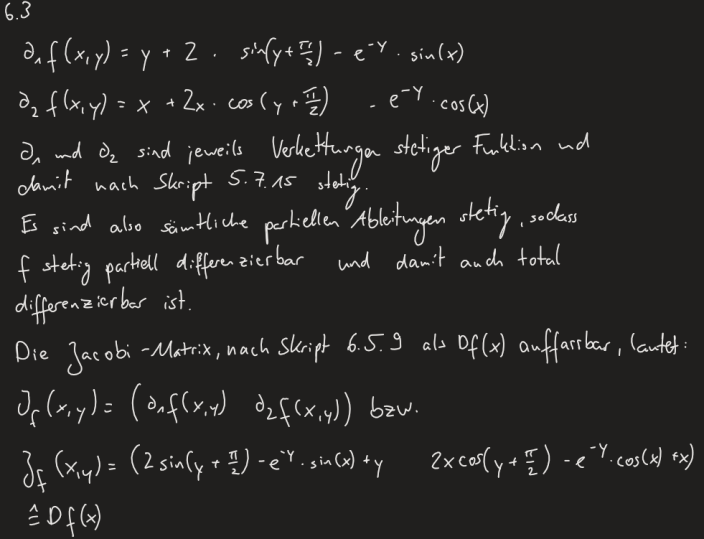
\includegraphics[scale=0.6]{ h3_1 }

\bigskip
\noindent b) 
Da sin(y  + $\frac{\pi}{2}$) = cos(y) schreiben wir die Funktion passend um.
Wir berechnen den Gradienten wie folgt:
\begin{align*}
    \triangledown f(x, y) &= \begin{bmatrix}
        \frac{\partial f}{\partial x} (xy + 2x * cos(y) + e^{-y} * cos(x) \\        
        \frac{\partial f}{\partial y} (xy + 2x * cos(y) + e^{-y} * cos(x)
                            \end{bmatrix}
                            (x, y) \\ 
                          &= \begin{bmatrix}
                              y + 2 * cos(y) - e^{-y} * sin(x) \\ 
                              x - 2x * sin(y) - e^{-y} * cos(x)
                          \end{bmatrix} 
                          (x, y) 
\end{align*}
Nun setzen wir (0, 0) ein:
\begin{align*}
    \triangledown f(0, 0) &= \begin{bmatrix}
       0 + 2 * cos(0) - e^0 * sin(0) \\ 
       0 - 2 * 0 * sin(0) - e^0 * cos(0)
    \end{bmatrix} \\ 
                          &= \begin{bmatrix}
                           2 * 1 - 1 * 0 \\ 
                           0 - 1 * 1
                          \end{bmatrix} \\ 
                          &= \begin{bmatrix}
                           2 \\ 
                           -1
                          \end{bmatrix}
\end{align*}
\end{document}

